%----------------------------------------------------------------------------------------
%	ARTICLE CONTENTS
%----------------------------------------------------------------------------------------

\section{Introduction}
	Le projet consiste à calculer la probabilité de non-remboursement d'un prêt bancaire.
	Le modèle retenu est LightGBM \cite{NIPS2017_6907}.
	

\section{Modèle}
	
	\subsection{Rappel sur les méthodes d'ensemble}
		Les méthodes d'ensemble sont une famille de modèle de machine learning se basant sur
		le principe simple suivant: plusieurs modèles que l'on peut qualifier de faibles, une fois combinés
		permettent d'obtenir de meilleurs prévisions. \cite{geron2017hands-on} \cite{scikit-learn} Les modèles combinés dans le modèle d'ensemble
		sont qualifiés d'apprenants faibles. Ces apprenants faibles peuvent être quelconques,
		du moment que leurs prévisions individuelles sont meilleures que de l'aléatoire.
		Dans le cadre de LightGBM, les apprenants faibles sont des arbres de décision.
		
		\begin{figure}
		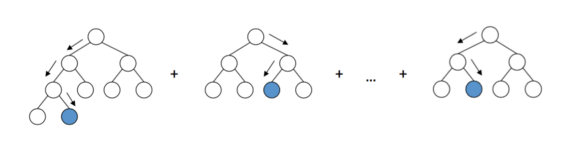
\includegraphics[width=\linewidth]{./figs/Boosting.png}
		\caption{Ensemble d'arbre de décision, le modèle final renvoie un 
				 résultat obtenu grâce à l'ensemble des apprenants faibles}
		\end{figure}
		
	\subsection{Arbre de décision}
		Un arbre de décision est un modèle représentant un ensemble de choix sous forme
		d'un arbre. 
		
		\begin{figure}[H]
		\centering
		\caption{Exemple d'arbre de décision.}
		\label{figure:decision_tree}
		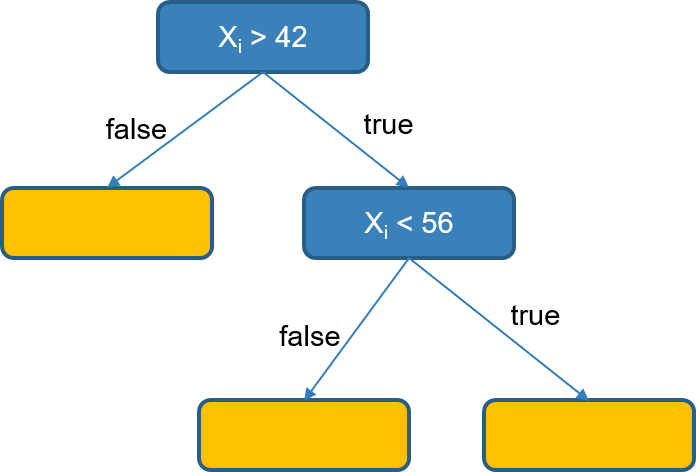
\includegraphics[scale=0.5]{DecisionTree.png}
		\end{figure}
		
		Les différentes décisions possibles sont situées aux niveaux des 
		feuilles de l'arbre (les feuilles étant les extrémités des branches de l'arbre) (cases orange sur la figure \ref{figure:decision_tree}),
		ces dernières sont finalement atteintes en fonction des décisions prisent à chaque
		n\oe ud de l'arbre (un n\oe ud correspond à la séparation de deux branches et donc 
		à une question (cases bleues sur la figure \ref{figure:decision_tree}))
		
		
	\subsection{Gradient boosting}
	
		Le boosting est une famille de méthodes d'ensemble dans lesquelles les apprenants faibles sont
		combinés de manière séquentielle (la sortie de la première couche d'apprenants est l'entrée
		de la couche n+1 \footnote{La première couche est en réalité une feuille unique 
		qui correspond à la moyenne des observations dans le cas d'une régression et qui est 
		la probabilité d'appartenance à une classe dans le cas d'une régression.
		($p=\frac{e^{\log(freq)}}{1 - e^{\log(freq)}}$ avec freq = frequence de la classe)}).
		Ainsi lors de l'entrainement du modèle, les apprenants
		n+1 vont <<apprendre à corriger>> les apprenants n et ainsi réduire le biais total du modèle d'ensemble.
		Cette correction est réalisée en affectant des poids à chaque individu en fonction de l'erreur produite
		et pris en compte lors de la création de l'arbre suivant.
		Ce processus se termine soit lorsque le nombre d'arbre préalablement spécifié est atteint, soit
		lorsque le modèle a atteint le minimum de la fonction de coût.	
		Chaque apprenant faible est également pondéré d'une constante appelé taux d'apprentissage (\emph{learning rate}) 
		permettant de réduire plus
		ou moins l'impact de chaque apprenant faible dans le résultat final.
		Le résultat final sera finalement la somme de tout les arbres de décision. 
		
		\subsubsection{Fonction de coût et algorithme d'optimisation}
		Lors de l'entrainement du modèle, ce dernier doit minimiser une fonction de coût global (équation \ref{loss}) \cite{NIPS2017_6907}\cite{geron2017hands-on},
		pour y parvenir, les différents apprenants faibles vont être mis à jour après chaque cycle
		de boosting. Pour mettre à jour les apprenants faibles dans la <<bonne direction>> (minimisation de 
		la fonction de coût), on calcule le gradient de la fonction de coût au travers des différents
		apprenants faibles. Dans le cas d'une classification de type binaire, la fonction de coût
		est une \emph{<<cross entropy loss function>>} voir équation \ref{loss}
		
		\begin{equation}
		\label{loss}
		H_p(q) = -\frac{1}{N} \sum_{i=1}^{N}y_i \cdot(p(y_i)) + (1 - y_i)\cdot \log(1 - p(y_i))
		\end{equation}
		
	\subsection{Avantages de LightGBM}
		LightGBM est une version optimisée de Gradient Boosting proposée par Microsoft. Les détails de
		ses particularités sont résumés dans sa documentation \footnote{\url{https://lightgbm.readthedocs.io/en/latest/Features.html}}
		En résumé, LightGBM tire ses avantages de deux techniques \cite{NIPS2017_6907}, la première est le \emph{<<Gradient-based One-side Sampling (GOSS)>>} et
		la seconde est le \emph{<<Exclusive Feature Bundling (EFB)>>}.
		
		\subsubsection{Gradient-based One-side Sampling}
		Cette méthode permet de réduire sensiblement le nombre d'observations tout en maintenant une bonne précision
		pour les arbres de décisions entrainés.
		Pour plus de détails, référez-vous à la publication originale \cite{NIPS2017_6907}
		
		\subsubsection{Exclusive Feature Bundling}
		Cette méthode permet de réduire le nombre de features en combinant certaines features non-exlusives.
		Cette méthode n'intervient que très peu dans ce projet car les données sont relativement de faibles
		dimensions (15 features dont une catégorielle donnant 33 features après transformation via One Hot Encoding.) les données
		de type matrice creuse peuvent être réduites par cette technique en combinant certaines features
		sous forme de nouvelles features (bundle) de dimensions réduites ($\#data \times \#feature$) vers ($\#data \times \#bundle$) 
	

\section{Métrique d'évaluation}
	La métrique finale utilisée est le score ROC AUC. (Receiver Operating Characteristic Area Under the Curve). \cite{ROC_AUC}
	%L'avantage d'utiliser ce score plutôt que la précision du modèle vient du fait que l'on 
	La courbe \emph{Receiver Operating characteristic} (ROC) est le graphique correspondant au taux de vrai positif
	en fonction du taux de faux positif pour tout les seuils de décision.(voir figure \ref{Courbe ROC}) 
	Sur ce graphique une classification naïve aléatoire correspond simplement
	à la diagonale, lorsque le modèle est meilleur que de l'aléatoire, on obtient une courbe située au-dessus
	de la diagonale. Ceci correspond à une meilleure séparation des deux distribution (voir figure \ref{distrib}
	
	
	\begin{figure}[H]
	\caption{Courbe ROC}
	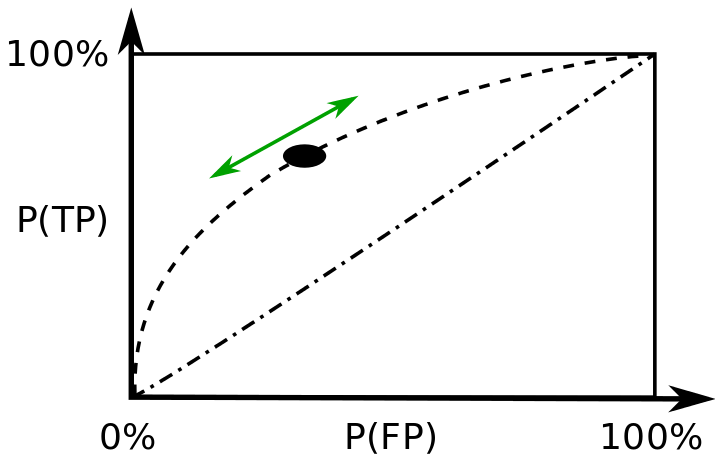
\includegraphics[scale=0.4]{./figs/ROC_1.png}
	\end{figure}
	\begin{figure}[H]
	\caption{Distribution des vrais positifs (TP) et vrais négatifs (TN). Le recouvrement des deux distributions
	 		 correspond aux faux négatifs (FN) et faux positifs (FP)}
	\label{distrib}
	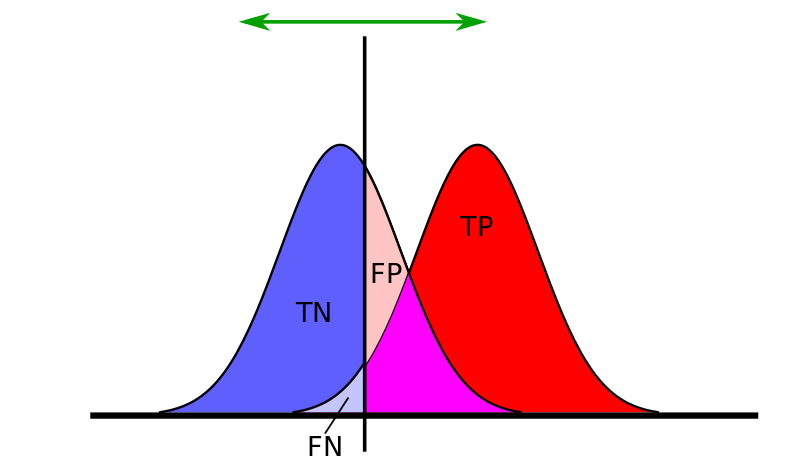
\includegraphics[scale=0.4]{./figs/ROC_2.png}
	\end{figure}
	Pour finalement calculer le score à proprement dit, on calcule l'aire sous la courbe (AUC) 
	(intégrale de la courbe sur l'ensemble). Ce score sera donc situé entre 0.5 (modèle aléatoire) et 1.0 modèle parfait.
	\begin{equation}
	\label{AUC}
	AUC = \int_{FP=0}^1 TP(FP) d(FP)
	\end{equation}
	Dans l'équation \ref{AUC}, TP correspond au taux de vrais positifs et PR correspond au taux de faux positifs.
	
\section{Interprétabilité du modèle}

	\subsection{Importance des variables}
	Pour interpréter les résultats du modèle, il est intéressant de savoir quelles variables rentrent en jeux lors de la prédiction.
	Pour connaitre l'importance des différentes variables, il est courant de calculer le nombre de split total engendrés par une variable.
	Plus le modèle crée des n\oe uds en utilisant une variable donnée plus cette dernière est importante. Il suffit alors de compter le
	nombre de n\oe uds dans tout les arbres de décision pour lesquelles une variable donnée est responsable du split pour obtenir une \emph{feature importance}.
	
	\subsection{Interprétation des résultats par additivité}
	Pour comprendre comment les scores finaux (probabilité de défaut d'un client) sont calculés, il est intéressant d'utiliser la librairie shap \cite{NIPS2017_7062} (SHapely Additive exPlanations). 
	Cette approche se base sur la théorie des jeux pour expliquer les sorties d'un modèle de machine learning. Ce système connecte l'allocation optimal de crédits
	avec une explication locale en utilisant les valeurs de Shapeley (voir théorie des jeux) et leurs extensions associées.
	
\section{Limites et améliorations possibles}
	Les limites et améliorations possibles sont plus liées aux données qu'au modèle. 
	En effet, certaines variables sont déséquilibrées dans le cas des données catégorielles 
	et asymétriques dans le cas des données numériques continues, ce déséquilibre est également vrai pour la cible. 
	Ce dernier point peut réduire la qualité des prédictions pour certaines classes sous-représentées et ne peut 
	être contourné que par une augmentation de la taille du jeu de données.
	
	Un autre problème avec les données utilisées est l'absence d'informations sur certaines variables,
	la nature abstraite de ces variables complique l'interprétation des résultats.